\documentclass{beamer}
\mode<presentation>
\usepackage{tikz}
\usepackage{graphicx}
\usepackage{tabu}
\usepackage{xcolor}
\usetikzlibrary{positioning}
\usetikzlibrary{calc}
\usetikzlibrary{backgrounds}
\usefonttheme{professionalfonts}
\usetheme{Orr}
\usepackage[orientation=portrait, size=custom, width=106.68 ,height=106.68 , scale=1.4]{beamerposter}
\usepackage{fontawesome}
\usepackage{booktabs}

\graphicspath{{./figures/}{./figures/generated/}{./figures/static/}}

\title{Reference-free Base Quality Score Recalibration for Sensitive Detection of Mutations}
\titlegraphic{
	
\includegraphics[width=.95\linewidth]{biodesign_logo.pdf}
	}
\date{3/22/19}
\author{Adam J Orr \inst{1,2} \faTwitter @AdamJOrr}
\institute{\inst{1} School of Life Sciences, Arizona State University \\
		   \inst{2} Biodesign Institute, Arizona State University}
\email{\faEnvelopeO \space ajorr1@asu.edu}
\website{\faLink \space   cartwrig.ht/lab/}

% \setlength{\topsep}{0pt}
% \setlength{\partopsep}{0pt}
\begin{document}

\begin{frame}{}
\begin{columns}[T]

%%%% Left side %%%%

\begin{column}[T]{.5\linewidth}

%%%%%%%%%%%%%%%%%%%

% \begin{block}{\large Abstract}
% DNA sequencing and methods that use the resulting sequencing data to detect genetic variation play an important role in many studies. Associated with the sequencing data are quality scores, which measure the probability of technical error at each base in the sequence. Statistical models for detecting variants utilize these scores to determine which sequences are reliable and which are not. However, these scores are often poorly calibrated and underestimate the probability of error, causing overconfidence in the results. Base quality score recalibration is a process to increase the accuracy of quality scores, which leads to more accurate inferences. However, current methods for base quality score recalibration require a reference genome and are inaccurate if the quality of the reference is poor. We present a reference-free method for base quality score recalibration which performs similarly to previous methods but can be used without a reference.
% \end{block}


\begin{block}{Introduction}

\begin{columns}
\column{.72\linewidth}
\begin{itemize}
\item Illumina sequencing reads contain errors
\item Errors make mutation detection difficult
\item Quality scores represent $P(error)$ on a phred scale.
\begin{displaymath}
P(error) = 10^{\frac{-Q}{10}}
\end{displaymath}
\begin{displaymath}
Q = -10\log_{10}{P(error)}
\end{displaymath}
\item Though quality scores are usually in the range \textbf{0 - 40}, to reduce the size of data files they are sometimes binned %into \textbf{7} bins 
\end{itemize}
\column{.25\linewidth}
\begin{tabular}{l l r} \toprule
\input{qtable1.tex}
\end{tabular}
\end{columns}
\end{block}

\begin{block}{\textcolor{black}{Methods:} Base Quality Score Recalibration - BQSR}
Base Quality Score Recalibration is a technique to undo binning \textit{and} improve calibration of the original quality scores.
However, \textbf{BQSR requires a reference genome and a database of variable sites}.
Our reference-free method uses the \texttt{lighter} software package to find erroneous bases rather than comparing the sequence to a reference.
\texttt{lighter} inspects the kmer spectrum to find errors and therefore doesn't require a reference.

\begin{figure}
\begin{center}

\textbf{GATK BQSR - Reference Required}

\begin{tikzpicture}[framed, align=center, sqnode/.style={rectangle,draw=black!60,fill=black!5,very thick,minimum size=1cm}, node distance = 4 cm]
	\node[sqnode] (sequencing) {Sequence};
	\node[sqnode] (alignment) [right = of sequencing] {Alignment};
	\node[sqnode] (ignorevar) [right = of alignment] {Ignore Variable Sites};
	\node[sqnode] (lookupref) [below = 2cm of alignment] {Assume Reference Mismatches Are Errors};
	\node[sqnode] (lnmodel) [below = 2cm of lookupref] {Predict Error Rate with Linear Model};
	\draw[line width=3mm,->] (sequencing) -- (alignment);
	\draw[line width=3mm,->] (alignment) -- (ignorevar);
	\draw[line width=3mm,->] (ignorevar) -- (lookupref);
	\draw[line width=3mm,->] (lookupref) -- (lnmodel);
\end{tikzpicture}
\end{center}
\end{figure}

\begin{figure}
\begin{center}

\textbf{Reference Free BQSR}

\begin{tikzpicture}[framed, align=center, sqnode/.style={rectangle,draw=black!60,fill=black!5,very thick,minimum size=1cm}, node distance = 4 cm]
	\node[sqnode] (sequencing) {Sequence};
	\node[sqnode] (kmer) [below = 2cm of sequencing] {Inspect Kmer Spectrum to Find Erroneous Bases with \texttt{lighter}};
	\node[sqnode] (lnmodel) [below = 2cm of kmer] {Predict Error Rate with Linear Model};
	\draw[line width=3mm,->] (sequencing) -- (kmer);
	\draw[line width=3mm,->] (kmer) -- (lnmodel);
\end{tikzpicture}

\end{center}
\end{figure}

\end{block}

\begin{block}{\textcolor{black}{Methods:} Hierarchical Linear Model}

The recalibration uses a hierarchical linear model to predict the true probability of error given a set of covariates.
Each covariate causes the predicted quality score to shift up or down from the predicted score one level above it in the hierarchy.

\begin{columns}
\column{.475\linewidth}

The relevant covariates are:
\begin{itemize}
	\item Read Group
	\item Original Assigned Quality Score
	\item Position in read and whether read is forward or reverse (Cycle)
	\item Base called and the prior base call (Context)
\end{itemize}

\column{.475\linewidth}

\begin{figure}
\begin{center}

\textbf{Hierarchical Linear Model}

\begin{tikzpicture}[align=center, sqnode/.style={rectangle,draw=black!60,fill=black!5,very thick,minimum size=1cm}, node distance = 4 cm]
	\node[sqnode,align=center,above,minimum size=16cm](rg) at (8,0){};
	% \draw[help lines] (0,0) grid (16,16);
	\node[](rglab) at (8,15){Read Group};
	\node[sqnode, align=center,above,minimum size=13cm,fill=gold!10](q) at (8,1){};
	\node[](qlab) at (8,12){Assigned Quality Score};
	\node[sqnode, minimum size = 5 cm,fill=maroon!10] at (5,6) {Cycle};
	\node[sqnode, minimum size = 5 cm,fill=maroon!10] at (11,6) {Context};
\end{tikzpicture}
\end{center}
\end{figure}
\end{columns}
\end{block}
%\textbf{Algorithm:} %For each base, record its read group, assigned quality score, cycle, context, and whether or not it was an error.
%Record the error rate of each read group, then subset each read group by the assigned quality score and calculate the error rate for each subset.
%Further subset these by 1) cycle and 2) context, and calculate the error rate for each subset.
\begin{block}{\textcolor{black}{Methods:} Algorithm}
Subset each base into groups according its covariates.
Use the mean base quality of the entire dataset as an initial prior. For each level in the hierarchy, the prior is normally distributed around the 
result of the previous level. Given this prior, find the maximum a posteriori (MAP) error rate and record the difference between the prior and the MAP.
This is similar to a penalized maximum likelihood. The recalibrated quality is the sum of these differences.

\vskip 2.2ex

\end{block}



% %%% Right Side %%%%
\end{column}
\begin{column}[T]{.5\linewidth}

%%%%%%%%%%%%%%%%%%%%%%%

\begin{block}{\textcolor{black}{Methods:} Evaluation}
\begin{itemize}
	\item CHM1 and CHM13 are human complete hydatidiform mole cell lines.
	% \item The moles are formed when a sperm combines with an egg containing no nucleus.
	% \item The sperm then undergoes mitosis to generate a completely homozygous cell mass.
	\item DNA from these two lines were mixed to generate a synthetic diploid dataset for benchmarking variant calling algorithms.
	\item We analyzed a small segment of Illumina sequencing reads aligned on Chromosome 1 and compared recalibrated quality scores generated using our method and the standard GATK method.
\end{itemize}
\end{block}

\begin{block}{\textcolor{black}{Results:} Similar performance, no reference or variants required}
\begin{center}
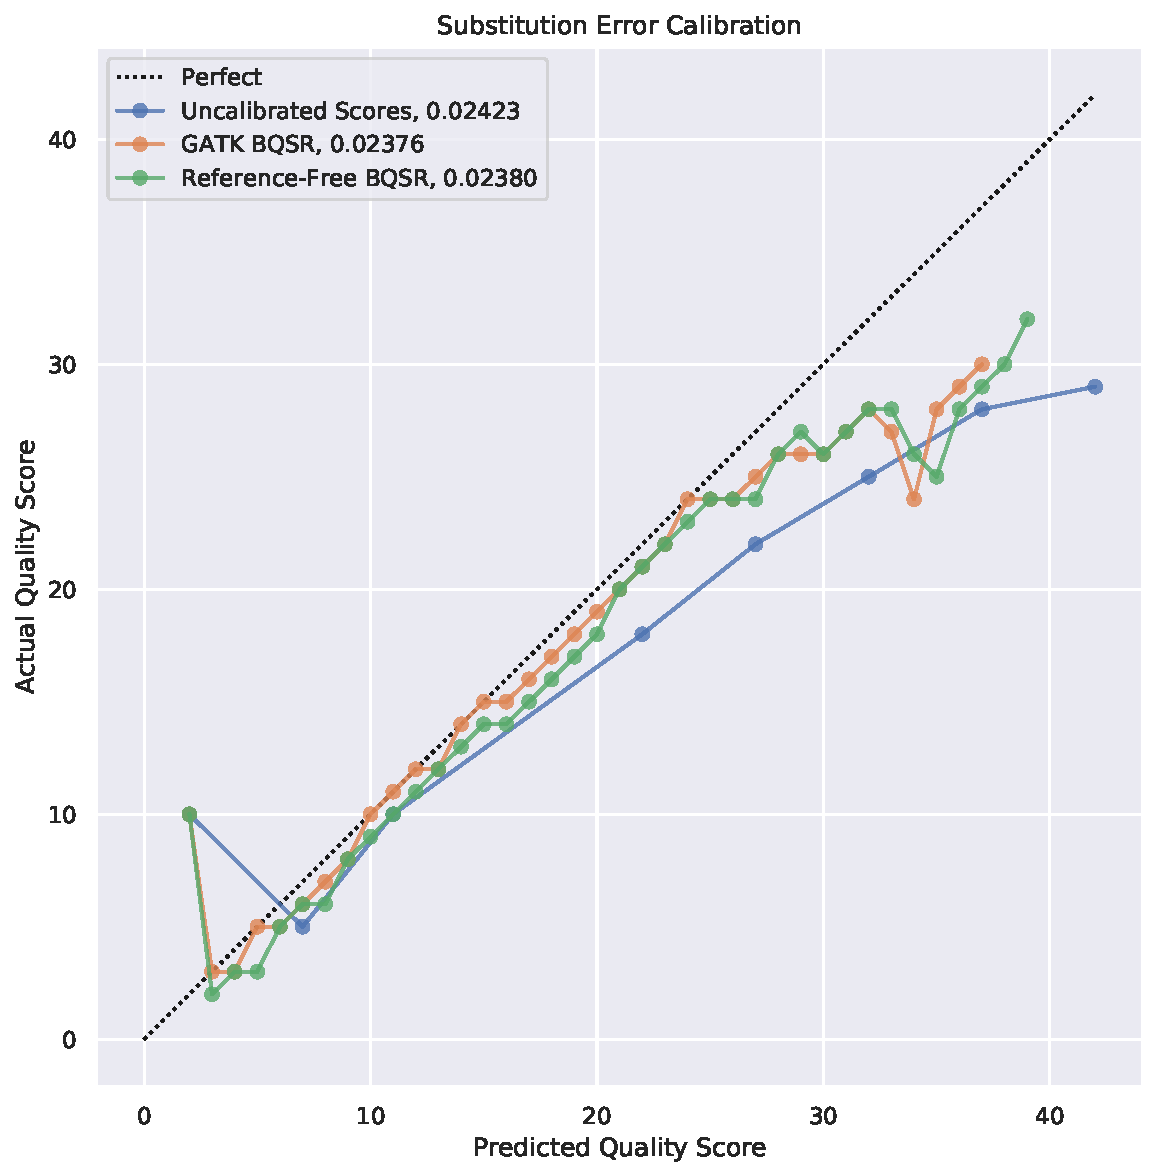
\includegraphics[width=.9\textwidth]{qualscores.pdf}
\end{center}
Both methods improve calibration and resolution, while our method has relaxed input requirements.
% The numbers in the legend are the Brier scores of each calibration method. The Brier score penalizes incorrect predictions,
% so a perfect prediction method will have a Brier score of 0. GATK BQSR improves the Brier score by $0.00047$ while our method
% improves the Brier score by $0.00043$. The peak at Q = 2 is because 2 is a reserved Illumina quality control mark and
% represents an invalid base.
\end{block}

\begin{block}{Next Steps}
\begin{itemize}
	\item Test performance against GATK BQSR with varying levels of false positives and false negatives.
	\item Simulate reads from a distant genome and compare performance with GATK BQSR.
	\item Linear model improvements
	\item Programming optimizations.
\end{itemize}
\end{block}


\begin{block}{Software}

\faicon{github} \url{https://github.com/adamjorr/kbbq}

\end{block}

\begin{block}{Acknowledgements}

% \begin{center}

\begin{columns}
%\column{.4\linewidth}
%This work is supported by grants NIH R01-HG007178 and NSF DBI-1356548.
\column{.27\linewidth}

\includegraphics[width=\linewidth]{lab_logo.pdf}
\column{.27\linewidth}

\includegraphics[width=\linewidth]{sols_logo.pdf}
\column{.3\linewidth}

\includegraphics[width=\linewidth]{biodesign_logo.pdf}
\end{columns}

% \end{center}

\end{block}

\end{column}
\end{columns}
\end{frame}

\end{document}